\documentclass[12pt]{article}


\usepackage[T1]{fontenc}
\usepackage{graphicx,color,amssymb,amsfonts,amsmath}
\usepackage{bbm,bm}
\usepackage[numbers]{natbib}
\usepackage{tikz}
\usepackage[left=2.5cm,right=2.5cm,top=3cm,bottom=3cm]{geometry}
\usepackage{alltt}
\newcommand{\ds}{\displaystyle}
\DeclareMathOperator{\logit}{logit}
\newcommand{\PP}{\mathbb{P}}
\newcommand{\ind}{\bm{\mathbbm{1}}}
\newcommand{\convL}{\overset{\mathcal{L}}{\rightarrow}}
\newcommand{\N}{\mathcal{N}}
\newcommand{\E}{\mathbb{E}}
\DeclareMathOperator{\diag}{diag}
\DeclareMathOperator{\Cov}{Cov}

\title{SNPSetSimulations: simulation of genotypic profiles under dependence}
\date{}
\author{Florian H\'{e}bert, Mathieu Emily, David Causeur}

\usepackage{Sweave}
\begin{document}
\Sconcordance{concordance:SNPSetSimulations.tex:SNPSetSimulations.Rnw:%
1 24 1 1 0 140 1}


\maketitle

	\section{Introduction}

\noindent This vignette provides help and examples of usage of the functions of the R package \texttt{SNPSetSimulations}. This package depends on packages {\bfseries lattice} \cite{lattice}, {\bfseries Matrix} \cite{Matrix} and, most importantly, {\bfseries GenOrd} \cite{GenOrd}.

	~

	\noindent In GWAS simulation studies, SNP-sets (or genes for simplicity) are often considered. These correspond to genotype data matrices; such a matrix can be denoted $\bm{X}$, its generic term being denoted $x_{ij}$. $x_{ij} \in \{0,1,2\}$ is the number of copies of the minor allele for the $i$-th individual and $j$-th SNP of the set. Strong and heterogeneous dependence structures are often observed among adjacent SNPs. Simulation studies must replicate such dependence structures to obtain realistic and reliable results.

	~

	\noindent The {\bfseries SNPSetSimulations} package aims at giving tools for generating simulated data related to case-control genome-wide association studies. In particular, it includes tools for simulating genotype and phenotype data under realistic scenarios. The package provides four functions: \texttt{levelplotSNP}, \texttt{PopulationSNPSet}, \texttt{PopulationPhenotype}, and \texttt{SampleSNPPhenotype}. Usage of each function will be explained hereafter, with examples given for each one.

	\section{Representing Within-Gene Dependence Structures}

	 The \texttt{levelplotSNP} function can be used to represent within-gene dependence structures as an heatmap. This function is based on the \texttt{levelplot} function from the {\bfseries lattice} package \cite{lattice}. Dependence is measured by Pearson's correlation coefficient. In the following example, we create a correlation matrix \texttt{Sigma} of size 20. \texttt{Sigma} has an autocorrelation structure with correlation parameter \texttt{rho} equal to 0.8. We finally plot this correlation matrix; see figure \ref{fig:heatmap} for the result.

	 \begin{alltt}
m = 20
rho = 0.8
Sigma = rho\^{}abs(outer(1:m,1:m,"-"))
levelplotSNP(Sigma)
	 \end{alltt}

 	\begin{figure}[!h]
 		\centering
 		\vspace*{-4em}
 		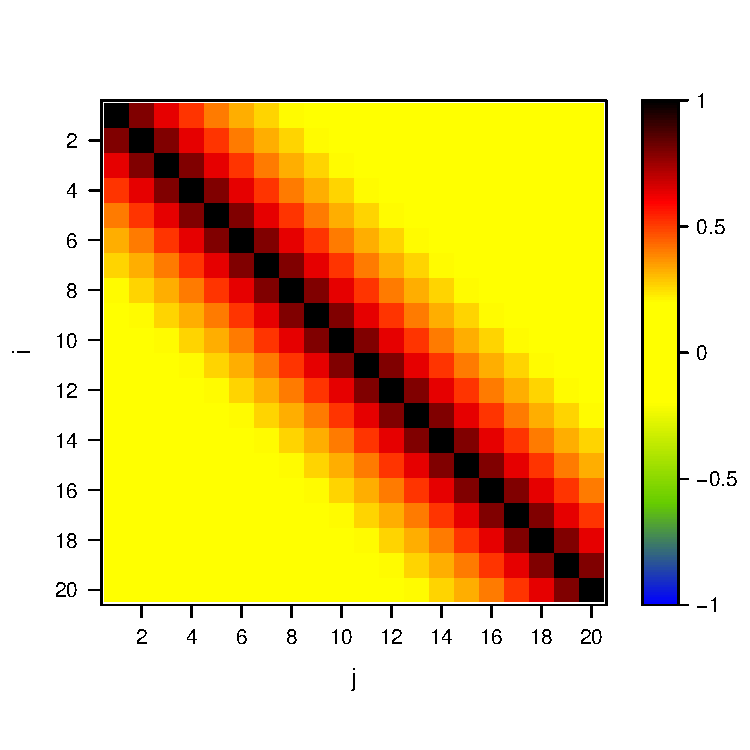
\includegraphics{heatmap.pdf}
 		\vspace*{-2em}
 		\caption{Heatmap of a correlation matrix obtained with function \texttt{levelplotSNP}}
 		\label{fig:heatmap}
 	\end{figure}

	 \noindent This function can be useful to display the dependence structure of a genotype matrix \texttt{X}. If such a matrix is loaded in the R environment, then it is sufficient to enter the following command:

	 \begin{alltt}
	levelplotSNP(cor(X))
	 \end{alltt}

 	 \noindent A legend is also displayed on the right of the plot. The colors are automatically chosen by the function on a continuous scale passing through yellow for null correlation, black for strong positive correlation, red for intermediate positive correlation, blue for strong negative correlation and green for intermediate negative correlation.

 	 \section{Generating Genotype Data}

 	 The function \texttt{PopulationSNPSet} provides a way of efficiently generating a matrix of genotypes for a population of \texttt{n} individuals and \texttt{m} SNPs according to given marginal distributions and within-gene dependence structure. This function can be used through several ways explicited by the following examples. In each example, the obtained matrix is stored in the variable \texttt{G}. Several arguments can be used:
 	 \begin{itemize}
 	 	\item \texttt{n}: the desired size of the simulated population
 	 	\item \texttt{Sigma}: the correlation matrix of the simulated SNP-set
 	 	\item \texttt{p}: a vector of minor allele frequencies (one value for each SNP); if this argument is given, genotypes are simulated according to Hardy-Weinberg equilibrium (HWE)
 	 	\item \texttt{marginal}: a list of marginal distributions. This argument can be used to generate genotypes under a chosen distribution, which can be different from HWE. Each element of the list is a vector of cumulative marginal probabilities. If the $k$-th SNP takes values 0, 1 and 2 with probabilities \texttt{p0}, \texttt{p1} and \texttt{p2}, the $k$-th vector of the list is \texttt{c(p0,p0+p1)}. The third cumulative probability is supposed to be equal to one and is not given
 	 	\item \texttt{X}: an observed SNP-set; this argument can be used to generate a population of \texttt{n} individuals with the same dependence structure and marginal distributions as those observed in the given SNP-set.
 	 \end{itemize}

 	 ~

 	 \noindent Simulation of \texttt{n = 100000} individuals, \texttt{m = 10} autocorrelated SNPs (correlation coefficient equal to 0.8), minor allele frequency \texttt{p = 0.4} for each SNP, under HWE:

 	 \begin{alltt}
G = PopulationSNPSet(n=100000,Sigma=0.8\^{}abs(outer(1:10,1:10,"-")),
 \hspace*{1.5em}p=rep(0.4,10))
 	 \end{alltt}

  	\noindent Simulation of \texttt{n = 100000} individuals, and \texttt{m = 10} autocorrelated SNPs (correlation coefficient equal to 0.8). Here, contrary to the first example, where only the MAF of each SNP was given, the complete marginal distribution of each SNP is given. Each SNP is supposed to be uniformly distributed (\emph{i.e.} the probability for an individual to get 0, 1 or 2 copies of the minor allele equals 1/3). These marginal distributions are given in the argument \texttt{marginal}, as a list of \texttt{m} elements. Each element of the list is a vector of cumulative probabilities.

 	\begin{alltt}
M = cbind(rep(1/3,10),rep(1/3+1/3,10))
M = lapply(1:nrow(M),function(i)\{M[i,]\})
G = PopulationSNPSet(n=100000,Sigma=0.8\^{}abs(outer(1:10,1:10,"-")),
\hspace*{2em}marginal=M)
 	\end{alltt}

 	\noindent Simulation of \texttt{n = 100000} individuals, and \texttt{m} SNPs according to marginal distributions and dependence structure given by an observed SNP set \texttt{Xobs}:

 	\begin{alltt}
G = PopulationSNPSet(n=100000,X=Xobs)
 	\end{alltt}

 	\noindent In the last example, the dependence structure, dimension (number of SNPs) and marginal distributions are automatically estimated on \texttt{Xobs}. One can check that the simulated data has the requested dependence structure and marginal distributions by comparing them to the observed SNP-set.

 	~

 	\noindent It is not trivial to generate correlated SNP data. Function \texttt{PopulationSNPSet} is based on modified versions of functions from the {\bfseries GenOrd} package \cite{GenOrd}, which gives tools for generating discrete data with given dependence structure and marginal distributions.

 	\section{Generating Phenotypes}

 	Once genotypes for a population are generated, a disease status corresponding to these genotypes can be generated using a specified model. The \texttt{PopulationPhenotype} function generates disease status conditionally to a matrix of genotypes \texttt{X} using a logistic model. Let $\bm{x_{i}}$ and $\bm{u_{i}}$ be the vector of genotypes and the optional vector of covariates of the $i$-th individual, respectively. Then the $i$-th individual is diseased with probability $\pi_{i}$ with
 	\begin{equation*}
 	\pi_{i} = \frac{\exp(\beta_{0}+\bm{u_{i}}'\bm{\alpha}+\bm{x_{i}}'\bm{\beta})}{1+\exp(\beta_{0}+\bm{u_{i}}'\bm{\alpha}+\bm{x_{i}}'\bm{\beta})}.
 	\end{equation*}
 	The disease status is then sampled as a Bernoulli variable with probability of success $\pi_{i}$. Cases are coded 1 and controls 0. Several parameters must be given:
 	\begin{itemize}
 		\item \texttt{X}: a matrix of genotype data, such as obtained with function \texttt{PopulationSNPSet}
 		\item \texttt{beta0}: the intercept of the logistic model
 		\item \texttt{beta}: the values of the non-zero coordinates of the vector $\bm{\beta}$ of the logistic model
 		\item \texttt{I}: the positions of the non-zero coordinates of $\bm{\beta}$
 		\item \texttt{U}: an optional matrix of covariates
 		\item \texttt{alpha}: the vector of effect parameters corresponding to the covariates
 		\item \texttt{mod}: a vector of characters giving the association model of each involved SNP - \texttt{"A"} for additive association (default), \texttt{"R"} for recessive association and \texttt{"D"} for dominant association.
 	\end{itemize}
 	In the following example, $\beta_{0} = -3$ and the 2nd and 7th coordinates of $\bm{\beta}$ are non-zero (both equal 0.2). The association between the disease and the involved SNPs corresponds to a recessive model. No covariates are used.

 	\begin{alltt}
Y = PopulationPhenotype(X=G,beta0=-3,beta=c(0.2,0.2),I=c(2,7),mod=c("R","R"))
 	\end{alltt}

	\noindent The association models can be mixed (\emph{e.g.} a SNP can be associated to the disease through an additive model and the other one through a recessive model). One can also desire to generate a phenotype that is independent from the SNPs. This corresponds to $\bm{\beta} = \bm{0}$; therefore, it can be done by setting \texttt{beta = 0} and \texttt{I = 1}. This function is not really supposed to be used on its own, but is necessary for the next function.

	\section{Generating Samples of Genotype and Phenotype Data}

	The most useful feature of this package is to generate samples of genotype data and corresponding disease status, \emph{i.e.} samples similar to that used in case-control GWAS. This is what provides the \texttt{SampleSNPPhenotype} function. Using a matrix of genotype data corresponding to a population (and an optional matrix of covariates), it generates the corresponding disease status using the \texttt{PopulationPhenotype} function. Then, it constructs a sample by randomly sampling a specified number of cases and controls. The result is given as a list of three elements: the first one is the genotype matrix of the sample, the second one is the vector of disease status corresponding to each row of the genotype matrix and the third one is the matrix of covariates corresponding to the sample. Several parameters must be given:
	\begin{itemize}
		\item \texttt{X}: a matrix of genotype data
		\item \texttt{beta0}: the intercept of the logistic model
		\item \texttt{beta}: the values of the non-zero coordinates of the vector $\bm{\beta}$ of the logistic model
		\item \texttt{I}: the positions of the non-zero coordinates of $\bm{\beta}$
		\item \texttt{n0}: number of controls
		\item \texttt{n1}: number of cases
		\item \texttt{U}: an optional matrix of covariates
		\item \texttt{alpha}: the vector of effect parameters corresponding to the covariates
		\item \texttt{mod}: a vector of characters giving the association model of each involved SNP - \texttt{"A"} for additive association (default), \texttt{"R"} for recessive association and \texttt{"D"} for dominant association.
	\end{itemize}

	\noindent In the following example, we generate a sample of 1,000 cases and 1,000 controls with the same genotype data and the same association model as in the example for function \texttt{PopulationPhenotype}:

	\begin{alltt}
		A = SampleSNPPhenotype(X=G,beta0=-3,beta=c(0.2,0.2),I=c(2,7),n0=1000,
		\hspace{2em}n1=1000,mod=c("R","R"))
	\end{alltt}

	\noindent The elements of the list are named \texttt{SNP}, \texttt{Phenotype} and \texttt{Covariates}. One can then compute association tests between each SNP and the phenotype. For example, using the $\chi^{2}$ test:
	\begin{alltt}
		Z = apply(A\$SNP,2,function(x)\{chisq.test(x,A\$Phenotype,correct=FALSE)\$p.value\})
	\end{alltt}

	\bibliographystyle{apalike}
	\bibliography{biblio}

\end{document}
